\begin{center}
	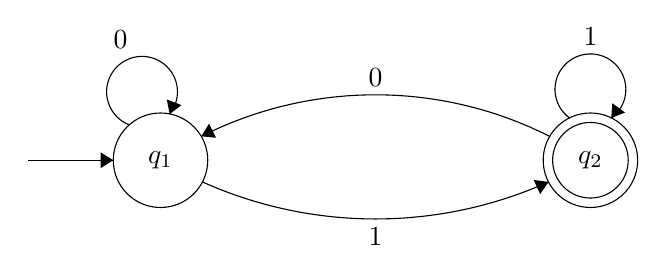
\begin{tikzpicture}[scale=0.2]
		\tikzstyle{every node}+=[inner sep=0pt]
		\draw [black] (24.2,-31) circle (3);
		\draw (24.2,-31) node {$q_1$};
		\draw [black] (51.5,-31) circle (3);
		\draw (51.5,-31) node {$q_2$};
		\draw [black] (51.5,-31) circle (2.4);
		\draw [black] (15.8,-31) -- (21.2,-31);
		\fill [black] (21.2,-31) -- (20.4,-30.5) -- (20.4,-31.5);
		\draw [black] (48.837,-32.378) arc (-65.8424:-114.1576:26.847);
		\fill [black] (48.84,-32.38) -- (47.9,-32.25) -- (48.31,-33.16);
		\draw (37.85,-35.23) node [below] {$1$};
		\draw [black] (26.787,-29.485) arc (116.84792:63.15208:24.496);
		\fill [black] (26.79,-29.48) -- (27.73,-29.57) -- (27.28,-28.68);
		\draw (37.85,-26.34) node [above] {$0$};
		\draw [black] (22.225,-28.757) arc (249.10435:-38.89565:2.25);
		\draw (21.67,-23.92) node [above] {$0$};
		\fill [black] (24.78,-28.07) -- (25.53,-27.5) -- (24.6,-27.14);
		\draw [black] (50.177,-28.32) arc (234:-54:2.25);
		\draw (51.5,-23.75) node [above] {$1$};
		\fill [black] (52.82,-28.32) -- (53.7,-27.97) -- (52.89,-27.38);
	\end{tikzpicture}
\end{center}
